
\chapter{Modeling} \label{ch:modeling}

To model the contact between the \gls{ee}'s tactile sensors, eight different model categories are present~\cite{articulated-hands-force-control-and-kinematic-issues} whereas the three most common ones within the field of robotics~\cite[Chapter 37]{handbook-of-robotics} are \gls{pwof}, \gls{hf} and the \gls{sf} model as shown in \figref{fig:contact-models}. \medskip

\begin{figure}[h]
	\centering
	\begin{subfigure}[b]{0.3\textwidth}
		\centering
		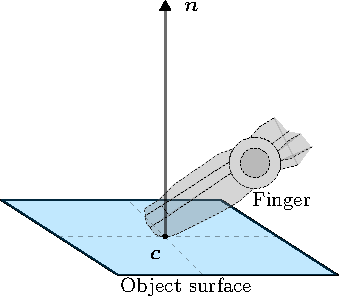
\includegraphics[width=\textwidth]{chapters/modeling/fig/contact-no-friction.pdf}
		\caption{\gls{pwof} in point \vec{c} with normal \vec{n}. \\\hspace{\textwidth} }
		\label{fig:pwof}
	\end{subfigure}
	\hfill
	\begin{subfigure}[b]{0.3\textwidth}
		\centering
		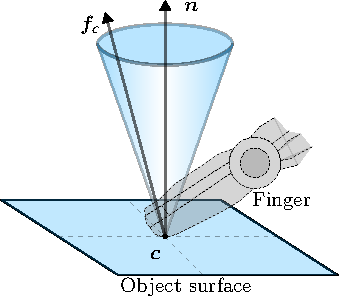
\includegraphics[width=\textwidth]{chapters/modeling/fig/hf.pdf}
		\caption{\gls{hf} in point \vec{c} with normal \vec{n} and contact force \mvar{\vec{f}_c}.}
		\label{fig:hf}
	\end{subfigure}
	\hfill
	\begin{subfigure}[b]{0.3\textwidth}
		\centering
		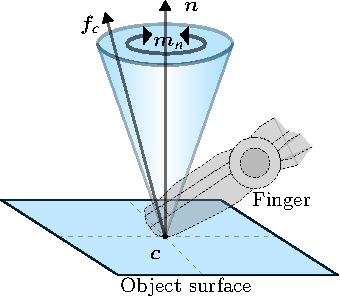
\includegraphics[width=\textwidth]{chapters/modeling/fig/sf.pdf}
		\caption{\gls{sf} in point \vec{c} with normal \vec{n}, contact force \mvar{\vec{f}_c} and friction moment \mvar{\vec{m}_n}.}
		\label{fig:sf}
	\end{subfigure}
	   \caption{The three most commonly used contact models.}
	   \label{fig:contact-models}
\end{figure}

% no friction
The \gls{pwof} model, as shown in \figref{fig:pwof}, can only represent forces along with the normal \mvar{\vec{n}\inR{3}} of the object's surface at the point of contact \mvar{\vec{c}\inR{3}} and thus the model does not support surface deformations between the two contacting objects. This model is applied in cases where very little deformation is present, along with the contact having a friction coefficient approximately equal to zero~\cite[Chapter 38]{handbook-of-robotics}.\medskip


% Hard finger
The \gls{hf} model, as shown in \figref{fig:hf}, is representative when the friction between objects is great enough to be significant, while the contact deformation is small enough to ignore friction moments and deformations~\cite[Chapter 38]{handbook-of-robotics}. To model the friction acting on the contact point a great number of methods exist, a common one being the Coulomb friction with different modifications depending on the use case~\cite{modelling-of-joint-friction-in-robotic-manipulators-with-gear-transmissions}. 
This model states that the frictional force acting on an object can be formulated as
%
\begin{equation}
	f_f = f_N \mu,
	\label{eq:coulomb-friction}
\end{equation}

with \mvar{f_f} being the Coulomb friction, \mvar{f_N} being the normal force in the point of contact and \mvar{\mu\in[0,1]} being the friction coefficient. One visualization of this linear relationship can be seen in the cones illustrated in \figref{fig:hf} and \figref{fig:sf}. These cones are referred to as friction cones, which for a hard finger model can be formulated as
%
\begin{equation} 
	\Chf = \left\{ \; f_c\; \middle|\; f_{t} \le \mu f_z,\; \mu f_z \ge 0 \; \right\} \qquad , \qquad f_t = \sqrt{f_x^2 + f_y^2}.
	\label{eq:hf}
\end{equation}
Here \mvar{f_c} is the magnitude of the contact force, \mvar{f_t} is the magnitude of the tangential force, \mvar{f_x}, \mvar{f_y} and \mvar{f_z} are the magnitudes of the \mvar{x}, \mvar{y} and \mvar{z} components of the contact force (\mvar{\vec{f}_c\inR{3}}) and \mvar{\mu} is the friction coefficient~\cite[Chapter 37]{handbook-of-robotics}. 
Thus by applying a contact force with a normal component i.e. \mvar{f_z} such that \mvar{f_z\mu} stays greater than the magnitude of the tangential component \mvar{f_t}, the friction force will remain great enough to ensure neither object slips. Visually this is the case when the contact force \mvar{\vec{f}_c} stays within the friction cone, which is a grasp type referred to as force closure. A force that commonly contributes significantly to the tangential force is gravity when the object is held purely through friction. \medskip

% The angle of the friction cone \mvar{\beta} can be computed based on \mvar{\mu} as
% %
% \begin{equation} 
% 	\beta = \tan\inv (\mu).
% 	\label{eq:hf-cone-angle}
% \end{equation}
% Soft finger
The \gls{sf} model, as shown in \figref{fig:sf}, is used to represent scenarios where both friction and surface deformations are great enough to be impactful in the behavior of the system. Due to deformations of the finger, an additional torsional moment about the contact normal will be present~\cite[Chapter 38]{handbook-of-robotics}. While an analytical formulation for the \gls{sf} relation depends on the pressure distribution inside the contact, and can only be derived for a limited number of special cases, the general case is approximated using 
%
\begin{equation} 
	\Csf = \left\{ \; f_c \; \middle| \; f_t^2 + \frac{m_n^2}{e_n^2} \le \mu^2 P^2 \right\} \qquad , \qquad f_t = \sqrt{f_x^2 + f_y^2}.
	\label{eq:sf}
\end{equation}
This formulation forms an ellipsoid $\Csf$ describing the relation between the tangential force \mvar{\vec{f}_t\inR{3}} and friction moment \mvar{\vec{m}_n \inR{3}}. Here \mvar{f_c} is the magnitude of the contact force, \mvar{f_t} is the magnitude of the tangential force, \mvar{m_n} is the magnitude of the frictional moment, \mvar{e_n} is the eccentricity parameter i.e. the height of the aforementioned ellipsoid, \mvar{\mu} is the friction coefficient and \mvar{P} is the magnitude of the pressure applied from the contact point along the contact normal \vec{n}~\cite{practical-force-motion-models-for-sliding-manipulation, soft-finger-model-with-adaptive-contact-geometry-for-grasping-and-manipulation-tasks}. \medskip

Based on the contact model categories described above, the most representative is the \gls{sf} models since these can provide descriptions of the contact surface shape, and thus enable the reconstruction of the contact shape from the application of a force distribution~\cite{contact-mechanics} i.e. the \gls{iep}. Furthermore, friction is crucial to manipulate objects in hand, which is also provided by these models. An illustration of the system as a \gls{sf} with friction cone and pressure distribution can be seen in \figref{fig:friction-contact-distribution}, while \figref{fig:force-closure-model} shows the model enabling force closure i.e. the composite wrench cone contains the entire wrench space so that any external wrench \vec{w_{\text{ext}}} on the body can be balanced by contact forces~\cite{modern-robotics-mechanics-planning-and-control}.
%
\begin{center}
    \renewcommand{\arraystretch}{1.2}
    \begin{minipage}{.48\linewidth}
        \vspace{0pt}
        \centering
        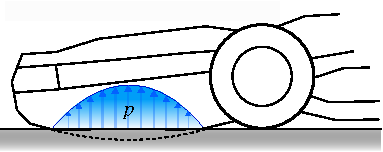
\includegraphics[width=.95\textwidth]{chapters/modeling/fig/contact-surface.pdf}%
        \vspace{0.6cm}
        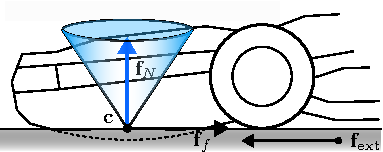
\includegraphics[width=.95\textwidth]{chapters/modeling/fig/friction-cone-schematic.pdf}%
    \end{minipage}%
    \hfill%
    \begin{minipage}{.48\linewidth}
        \vspace{0pt}
        \centering
        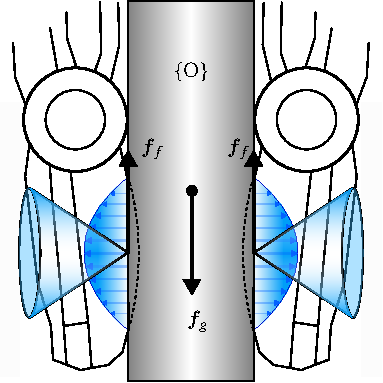
\includegraphics[width=.95\textwidth]{chapters/modeling/fig/force-closure-schematic.pdf}
    \end{minipage}%
    %    
    \vspace{15pt}
    %
    \begin{minipage}[t]{.48\linewidth}
        \vspace{0pt}
        \captionsetup{type=figure}
        \captionof{figure}{Contact pressure distribution and friction cone for a \gls{sf} model in the context of a robotic finger.}
        \label{fig:friction-contact-distribution}
    \end{minipage}%
    \hfill%
    \begin{minipage}[t]{.48\linewidth}
        \vspace{0pt}
        \captionsetup{type=figure}
        \captionof{figure}{Contact pressure distribution and friction cone causing force closure to prevent the object \robframe{O} from falling due to gravity.}
        \label{fig:force-closure-model}
    \end{minipage}%
\end{center}
When modeling the kinematics of a humanoid gripper with frame \mvar{\robframe{H}\inR{4\times 4}} in world frame \mvar{\robframe{W}\inR{4\times 4}} interacting with an object with frame \mvar{\robframe{O}\inR{4\times 4}} the different parameters and modeling are necessary. In this system the object with position \mvar{\vec{p}\inR{3}} and pose \mvar{\vec{u}\inR{6}}, with the orientation either being represented as a four-dimensional quaternion or a three-dimensional Euler angle, makes contact with the gripper in points \mvar{\vec{c}_i\inR{3}}. Said contact points have frames \mvar{\robframe{C}_i\inR{4 \times 4}} with axes \mvar{\rlist{\vec{n}_i,\vec{t}_i,\vec{o}_i}\subset \R^{3}}, where \mvar{\vec{n}_i\inR{3}} points perpendicular to the contact plant towards the object while the remaining are contained within the contact plane. The twist of \robframe{O} described in \robframe{W} is denoted $\vec{\nu} = \rvec{\vec{v}^\T \vsep \vec{\omega}^\T}^\T\inR{6} $ while the non-contact wrench i.e. the wrench caused by external forces such as collisions with the environment and gravity, is $\vec{w} = \rvec{\vec{f}^\T \vsep \vec{m}^\T}^\T\inR{6}$. \medskip

The gripper has $n_q$ joints named $\vec{q} = \rvec{q_1  \vsep q_2  \vsep \dots  \vsep q_{n_q}}^\T\in\R^{n_q}$ with loads $\vec{\tau} = \rvec{\tau_1  \vsep\tau_2  \vsep\dots  \vsep\tau_{n_q} \vsep}^\T\in\R^{n_q}$.




% About the object $\{O\}$ where the external force is represented as gravity which is a common occurrence.

% Within these figures $p(r)$ is the pressure distribution often as a function of the contact surface's radius $r$ assuming a non-conforming contact case. $\vec{f}_N$ is the normal force of the object acting on the \gls{ee} in the contact point $\vec{c}$, $\vec{f}_f$ is the friction force opposing the external force $\vec{f}_{\text{ext}}$ which often comes in the form of gravity $\vec{f}_g$ as see in \figref{fig:force-closure-model}.

% make the object identical to the one in the previous figure + finger tip contour from contact models
% see notion page

\begin{figure}[h]
	\begin{small}
		\begin{center}
			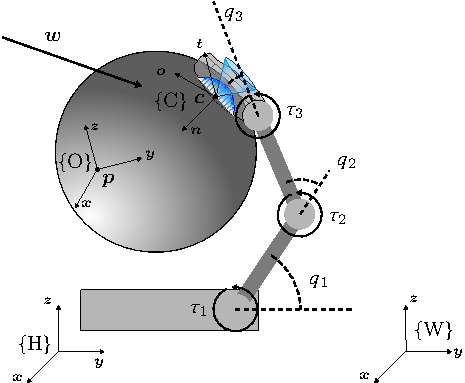
\includegraphics[width=0.6\textwidth]{chapters/modeling/fig/sys-schematic.pdf}
		\end{center}
		\caption{The model of the world representation for this project.}
		\label{fig:full-system-model}
	\end{small}
\end{figure}

% With the contact model described a segment of the kinematic tree of the \gls{ee} can be seen in \figref{fig:full-system-model}. Here $q_{thi}$ is the angle of the $i$'th joint in the thumb which here is the only finger depicted, $\boldsymbol{\tau}_{thi}$ is the torque exerted by said joint, $\{W\}$ is the world frame, $\{O\}$ is the object's frame and $\{H\}$ is the robotic hand's frame. 

While only a single finger here is illustrated the naming conventions and representations simply scale to all the \gls{ee}'s \gls{dof}s.\medskip

In this system, the twists and wrenches of contact point \mvar{\vec{c}_i\inR{3}} on the object and hand, given in contact frame \mvar{\robframe{C}_i} is referred to as \mvar{\vec{\nu}_{i,\xi}\inR{6}} and \mvar{\vec{w}_{i,\xi}\inR{6}}, with \mvar{\xi = \rlist{\text{obj}, \text{hnd}}}, respectively. Given multiple \gls{ee}s multiple contact points will exist, each with its twist and wrench. By concatenating these, two vectors can be expressed containing all twists and wrenches of the grasp, one for the object and one for the hand. These vectors are referred to as 
%
\begin{equation}
	\vec{\nu}_{c,\xi} = \rvec{\vec{\nu}_{1,\xi}^\T \vsep \vec{\nu}_{2,\xi}^\T \vsep \ldots \vsep \vec{\nu}_{n_c,\xi}^\T}^\T \inR{6\cdot n_c}
	\label{eq:all-twists}
\end{equation}
%
and
\begin{equation}
	\vec{w}_{c,\xi} = \rvec{\vec{w}_{1,\xi}^\T \vsep \vec{w}_{2,\xi}^\T \vsep \ldots \vsep \vec{w}_{n_c,\xi}^\T}^\T \inR{6\cdot n_c}
	\label{eq:all-wrenches}
\end{equation}
%
respectively. \medskip

These definitions are used to describe and analyze the kinematics of grasping and the forces involved in holding an object, also referred to as \gls{gk}. Within \gls{gk} two matrices are of special interest: the grasping matrix \mat{G} and the hand Jacobian \mat{J}. The grasping matrix describes the transformation between a twist or wrench of the object in world frame \robframe{W} to the contact frames of each contact point \mvar{ \robframe{C}_i \mfor i = 1,2,\ldots,n_c} where \mvar{n_c} is the number of contact points. The grasp matrix thus can be expressed as
\begin{equation}
	\mat{G} = \rvec{ \mat{G}_1 \vsep \mat{G}_2 \vsep \mat{G}_1 \vsep \cdots \vsep \mat{G}_{n_c}},
	\label{eq:grasp-matrix-def}
\end{equation}
where \mvar{\mat{G}_i \inR{6\times 6} \mfor i = 1,2,\ldots,n_c} and thus \mvar{\mat{G}\inR{6\times 6\cdot n_c}}. Using this grasp matrix, the object wrench and twist can be computed in all contact frames as
%
\begin{equation}
	\vec{\nu}_{c,\text{obj}} =  \mat{G}^\T \vec{\nu} \mspa \mand \mspa \vec{w}_{c,\text{obj}} =  \mat{G}^\T \vec{w}.
	\label{eq:grasp-matrix-twist}
\end{equation}
%
While the grasp matrix can be used to describe the transformation from world frame to contact frame, the hand Jacobian describes \gls{ee} velocity and force, given some joint velocities and torques
% 
\begin{equation}
	\vec{\nu}_{c,\text{hnd}} = \mat{J}^\T \dot{\vec{q}} \mspa \mand \mspa \vec{w}_{c,\text{hnd}} = \mat{J}^\T \vec{\tau}
	\label{eq:hand-jacobian-velocity}
\end{equation}
%
The hand Jacobian here 
\begin{equation}
	\vec{w}_{c,\text{hnd}} = \mat{J}^\T \vec{\tau}
	\label{eq:hand-jacobian-force}
\end{equation}

The grasp matrix which relates the object's twist \vec{\nu} to the twist of each contact point

see the robotics handbook and make sure to fully grasp partial, complete and grasp matrix

\textcolor{red}{Describe the grasp matrix and hand jacobian and how these can be used to transform from between frames both related to twist and wrench.}

To determine which methods best describe the models presented above for this project, the \gls{sota} will be presented in \chapref{ch:state-of-the-art}.


% grasp calculus
	% The hand-book-of-robotics chapter 38